\chapter{Proposta}

\section{Modelo Teórico} 

Segundo \cite{quteprints2107}, os modelos conceituais são utilizados para facilitar, sistematizar e auxiliar o processo de engenharia de sistemas de informação. \cite{wand_research_2002} mencionam em seu trabalho que os modelos conceituais descrevem objetos de sistemas de algum domínio em termos semânticos, utilizando uma linguagem abstrata, porém formalizada. Neste trabalho sera apresentado um modelo conceitual de um sistema de informação fundamentado na teoria da autoridade cognitiva de \cite{Wilson1983}.

A teoria da Autoridade Cognitiva, como explicado anteriormente é uma teoria social sobre o modo como as pessoas identificam, reconhecem e atribuem autoridade umas às outras (\cite{Wilson1983}). Um conjunto de regras e diretrizes foram criados para apoiar a verificação coletiva de qualidade da informação em redes sociais online. Para isso foram propostos 3 elementos que serviram de base para todas as articulações propostas:

\begin{enumerate}
    \item \textbf{Atores}: são os indivíduos na rede, podendo representar pessoas, empresas, instituições, organizações e artistas. O elemento ator deve possuir no mínimo atributos listados na tabela \ref{tab:atributos_ator}.
    \begin{center}
        \begin{table}[!htp]
            \centering
            \caption{Atributos de um ator}
            \label{tab:atributos_ator}
            \begin{tabular}{|p{4cm}|p{10cm}|}
                \cline{1-2}
                \multicolumn{2}{|c|}{Ator}  \\
                \hline
                Identificador & Código único utilizado para identificar um elemento na rede\\
                \hline
                Autoridades Cognitivas recebidas & Lista com as AC recebidas de outros atores na rede\\
                \hline
                Autoridades Cognitivas concedidas & Lista com as AC concebidas a outros atores na rede\\
                \hline
            \end{tabular}
        \end{table}    
    \end{center}
    
    
    \item \textbf{Objetos}: São as informações postadas pelos atores na rede. A tabela \ref{tab:atributos_objeto} ilustra esses atributos. Nos exemplos e explicações mostradas neste texto iremos utilizar URLs\footnote{"Abbreviation for uniform resource locator: a website address". Segundo a definição do dicionário de Cambridge: https://dictionary.cambridge.org/dictionary/english/url. Acessado em 24 de Janeiro, 2018.}\footnote{Tradução do autor: "Abreviação para Localizador Uniforme de Recursos: um endereço de webisite.} como identificador dos objetos. 
    \begin{center}
        \begin{table}[!htp]
            \centering
            \caption{Atributos de um objeto}
            \label{tab:atributos_objeto}
            \begin{tabular}{|p{4cm}|p{10cm}|}
                \cline{1-2}
                \multicolumn{2}{|c|}{Objeto}  \\
                \hline
                Identificador & Código único utilizado para identificar um elemento na rede, URLs são um bom exemplo de indicadores que podem ser utilizados\\
                \hline
                Palavras-chave & Lista com as palavras-chave recebidas de outros atores na rede\\
                \hline
                Classificação & Lista com as classificações recebidas de outros atores na rede\\
                \hline
            \end{tabular}
        \end{table}    
    \end{center}
    
    \item \textbf{\emph{Tags} (rótulos, em Português)}: são as palavras-chave que os atores utilizam para atribuição de autoridades cognitivas entre si, e para descrever e/ou categorizar objetos como pode-se observar na tabela \ref{tab:atributos_objeto}. 
    Apesar do grande papel que possui na organização e classificação dos objetos, as \emph{tags} não possuem muitos atributos, se mantendo apenas com um atributo texto de tamanho limitado que conterá apenas um rótulo. A tabela \ref{tab:atributos_tag} ilustra este elemento.
    \begin{center}
        \begin{table}[!htp]
            \centering
            \caption{Atributos de uma tag}
            \label{tab:atributos_tag}
            \begin{tabular}{|p{4cm}|p{5cm}|}
                \cline{1-2}
                \multicolumn{2}{|c|}{Tag}  \\
                \hline
                Termo & Texto com tamanho limitado\\
                \hline
            \end{tabular}
        \end{table}    
    \end{center}
\end{enumerate}

Além dos elementos estruturais, o modelo segue algumas diretrizes que serão apresentadas a seguir. Essas diretrizes regem as interações entre os elementos apresentados.
% em forma de URL\footnote{"Abbreviation for uniform resource locator: a website address". Segundo a definição do dicionário de Cambridge: https://dictionary.cambridge.org/dictionary/english/url. Acessado em 24 de Janeiro, 2018.}\footnote{Tradução do autor: "Abreviação para Localizador Uniforme de Recursos: um endereço de webisite.}

%----------------------------------------------------------------------------------------------------------------------------------------
\subsection{Autoridade Cognitiva é relativa a uma  área de interesse}

Em alguns assuntos uma pessoa pode ser autoridade, entretanto ela pode não saber nada sobre outros assuntos longe de sua área de conhecimento (\cite{Wilson1983}). Portanto, os indivíduos na rede devem ser capazes de atribuir uns aos outros zero ou mais áreas de expertise: "A" pode atribuir autoridade em matemática para "B" (exemplo na figura \ref{fig:diagrama_relacionamento}). Isso também significa que um indivíduo possui a capacidade declarar seus interesses, pois somente ele sabe qual área possui afinidade. 

A figura \ref{fig:diagrama_auto-atribuida} demonstra a auto-atribuição de duas expertises utilizando \emph{tags} (que são representadas com o símbolo de cerquilha seguido por uma palavra). Note que o exemplo não ilustra uma Autoridade Cognitiva pois não foi reconhecido por ninguém. Para que exista uma AC uma expertise precisa ser reconhecida por outro ator.

\begin{figure}[ht]
\centering
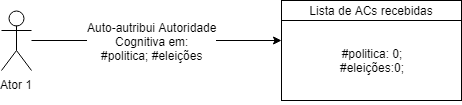
\includegraphics[scale=0.65]{4-proposta/diagrama_auto-autribuida.png}
\caption{Auto-atribuição de Autoridade Cognitiva.}
\label{fig:diagrama_auto-atribuida}
\end{figure}

Além de atribuir áreas de interesse uns aos outros, os atores podem utilizar \emph{tags} em formas de palavras-chave para atribuir uma descrição a um objeto na rede, como mostrado na figura \ref{fig:diagrama_palavras-chave}. As descrições propostas pelos atores podem auxiliar na identificação de áreas de interesse, auxiliando também na recuperação de informações por outros atores da rede (\cite{pereira_folkauthority:_2008}).

\begin{figure}[ht]
\centering
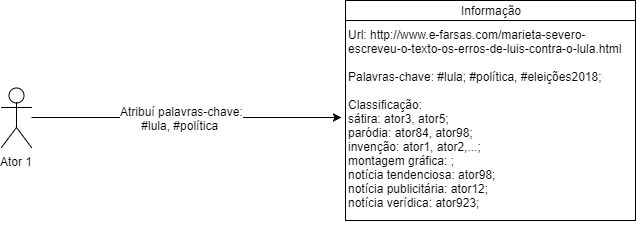
\includegraphics[scale=0.65]{4-proposta/diagrama_atribuicao_tags.png}
\caption{Atribuição de palavras-chave a uma informação.}
\label{fig:diagrama_palavras-chave}
\end{figure}

%----------------------------------------------------------------------------------------------------------------------------------------

\subsection{Autoridades Cognitivas possuem diferentes níveis}

Uma quantidade de AC pode ser possuída, seja ela pouca ou muita (\cite{Wilson1983}). Ou seja, iremos tratar AC como objetos que podem ser dados ou recebidos e uma quantidade destes pode ser possuída. Wilson ainda conclui que as pessoas, normalmente, expressam AC por meio de bases indiretas e que nem sempre é possível demonstrar essa autoridade em um valor ou escala mensurável. Portanto, propõe-se que existam duas listas: \textbf{lista de Autoridades Cognitivas recebidas}, que gerencia a AC que um indivíduo recebe de outro na rede; e uma \textbf{lista de Autoridades Cognitivas concedidas}, que gerencia as ACs que foram distribuídas para outro indivíduo na rede. Dessa forma é possível compilar um índice global que aumenta conforme outros usuários da rede reconhecem sua AC ( como ilustrado na figura \ref{fig:diagrama_relacionamento}). Esse índice pode ser analisado por outros atores e utilizado como indicador para saber se uma Autoridade Cognitiva é ou não reconhecida pelos seus pares. 

\begin{figure}[ht]
\centering
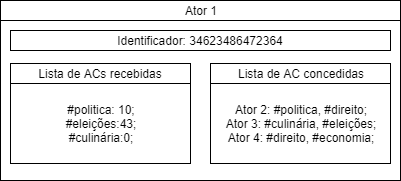
\includegraphics[scale=0.7]{4-proposta/diagrama_concebidos_recebidos.png}
\caption{Autoridades Cognitivas recebidas e concebidas.}
\label{fig:diagrama_recebidas_concebidas}
\end{figure}

Na figura \ref{fig:diagrama_recebidas_concebidas} percebe-se que na lista de ACs recebidas as áreas de interesse possuem valores destintos ilustrando o que acontece quando vários atores reconhecem a autoridade em uma mesma área. No assunto "eleições" o "Ator 1" foi reconhecido por 43 pessoas demonstrando um alto nível se comparado aos outros assuntos. Nota-se também que no assunto "culinária" o ator não foi reconhecido por ninguém, ilustrando um assunto que ele tem interesse porém ainda não é uma Autoridade Cognitiva para nenhum usuário na rede.



%----------------------------------------------------------------------------------------------------------------------------------------

\subsection{Autoridade Cognitiva envolve um relacionamento}

De acordo com \cite{Wilson1983} para a atribuição de AC é necessário o envolvimento entre no mínimo dois elementos. Além disso, \cite{pamela_j._mckenzie_justifying_2003} conclui que uma autoridade não é uma questão de inteligência ou especialidade, é uma questão de afinidade, confidência e admiração. Nota-se que não podemos considerar apenas como um relacionamento entre pessoas, pois é possível reconhecer autoridades em livros, instituições, instrumentos e organizações (\cite{soo_young_rieh_credibility_2010}). Ou seja, o ato de atribuir autoridade a alguma pessoa ou instituição é subjetiva e pessoal. O que pode ocasionar em erros por parte de quem reconhece uma autoridade, portanto é necessário uma checagem por parte de quem recebe, aceitando ou não ser AC sobre determinado assunto. Esse relacionamento é representado na figura \ref{fig:diagrama_relacionamento}.

\begin{figure}[ht]
\centering
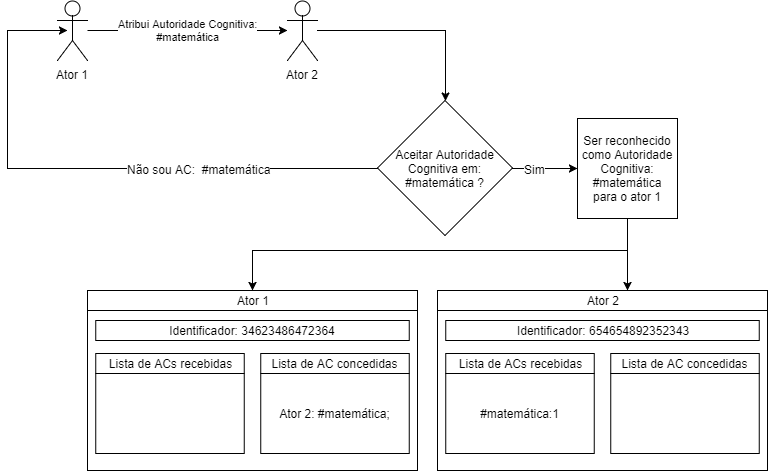
\includegraphics[scale=0.58]{4-proposta/diagrama_relacionamento.png}
\caption{Atribuição de Autoridade Cognitiva.}
\label{fig:diagrama_relacionamento}
\end{figure}

A figura \ref{fig:diagrama_relacionamento} demonstra ainda que AC é \textbf{unidirecional}: o fato de "A" ser uma autoridade para "B", não implica que "B" seja também uma autoridade para "A", mesmo que essa condição seja também possível (\cite{pereira_folkauthority:_2008}). Também é importante discutirmos sobre uma autoridade que foi renovada por outro ator, por exemplo, em uma situação onde "Ator 2" aceitou previamente a AC em matemática reconhecida por  um "Ator 0" ou atribuindo essa AC em si mesmo. Neste caso o "Ator 2" não precisará aceitar novamente, pois já possui reputação no assunto, mesmo que ela seja 0 (zero). 

\begin{figure}[ht]
\centering
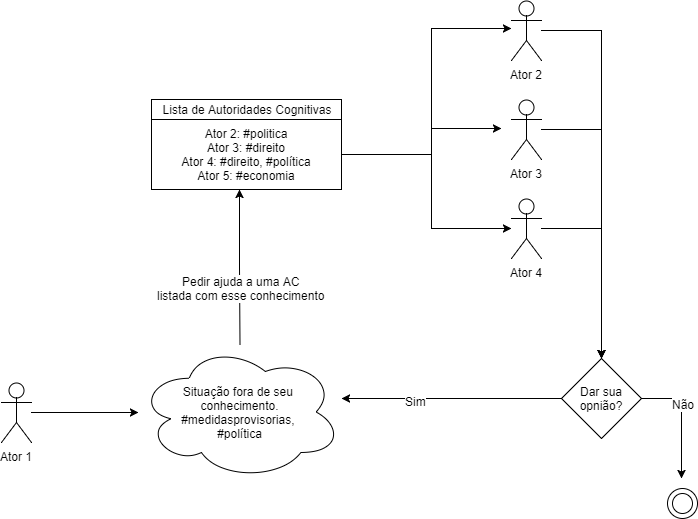
\includegraphics[scale=0.65]{4-proposta/diagrama_ajuda.png}
\caption{Solicitação de opinião para Autoridades Cognitivas.}
\label{fig:diagrama_ajuda}
\end{figure}

A partir do momento em que a relação de Autoridade Cognitiva é confirmada (proposta por quem reconhece e aceita por quem recebe), aquele que reconhece pode pedir ajuda para assuntos que são do interesse de quem aceitou a condição de AC. Uma AC não tem a obrigação de dar sua opinião sobre uma informação e pode ignorar a requisição. Esse relacionamento é ilustrado na figura \ref{fig:diagrama_ajuda}.

\begin{figure}[ht]
\centering
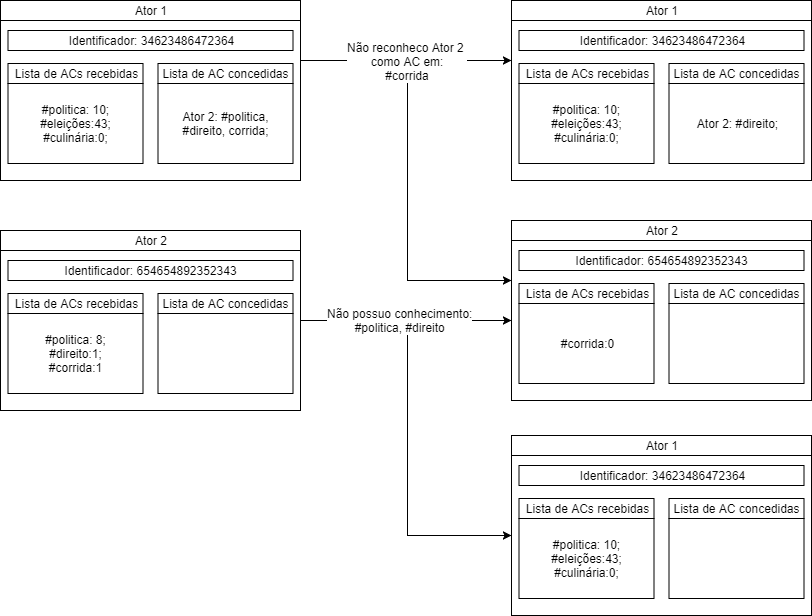
\includegraphics[scale=0.55]{4-proposta/diagrama_exclusao.png}
\caption{Exclusão de Autoridade Cognitiva.}
\label{fig:diagrama_exclusao}
\end{figure}

Um ator pode a qualquer momento reconsiderar uma AC atribuída por ele, assim como uma AC reconhecida pode renunciar uma Autoridade, como o ilustrado da figura \ref{fig:diagrama_exclusao}. O fato de um indivíduo "A" reconsiderar uma AC atribuída a um indivíduo "B", não significa que "B" não é mais uma AC, significa que o nível de AC de "B" diminuiu. Só é possível a eliminação total de um AC por parte do próprio indivíduo, pois uma Autoridade pode ser auto-atribuída. A figura \ref{fig:diagrama_exclusao} ainda mostra que mudança de de AC concebida ou recebida por parte de qualquer ator afeta os outros atores na rede.

%----------------------------------------------------------------------------------------------------------------------------------------

\subsection{Autoridades Cognitivas são diretamente relacionadas a credibilidade}

A influência de uma autoridade é aceitável pois esta é crível, digna de confiança (\cite{Wilson1983}). Portanto, além das diretrizes que permitem a identificação e organização das ACs devem existir mecanismos que permitam que os atores sinalizem confiança (ou desconfiança) nas informações compartilhadas na rede. 

O mecanismo proposto baseia-se na tipologia estudada por \cite{tandoc_defining_2017} que mapeia 6 formas de \emph{fake news}: (1) sátira; (2) paródia; (3) invenção; (4) montagem gráfica; (5) notícia publicitária; (6) notícia tendenciosa. Os atores devem ser capazes de classificar os objetos que trafegam na rede utilizando rótulos que representam os 6 tipos mapeados com a adição de mais um rótulo para expressar confiança: \textbf{notícia verídica}. A figura \ref{fig:diagrama_classificacao} representa esta ideia.

\begin{figure}[ht]
\centering
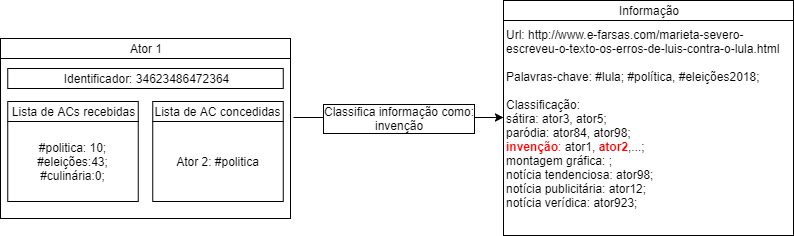
\includegraphics[scale=0.55]{4-proposta/diagrama_atribuicao_classificacao.png}
\caption{Classificação de um objeto na rede.}
\label{fig:diagrama_classificacao}
\end{figure}

Cada ator pode utilizar apenas uma classificação para cada objeto, sendo possível mudar posteriormente sua opinião. Essa regra busca evitar que alguns atores forcem uma classificação na rede.

Deve ser possível visualizar o índice completo da quantidade de atores que classificaram o objeto e qual classificação foi utilizada. Além disso priorizar a opinião dos atores considerados Autoridades Cognitivas no assunto em questão. Esse índice auxilia os outros atores da rede a identificar o objeto e decidirem por si mesmo qual a opinião deles sobre o mesmo.


%----------------------------------------------------------------------------------------------------------------------------------------

\section{Protótipo}

Este trabalho propõe o desenvolvimento de um sistema protótipo que implementará as diretrizes e fundamentos apresentados no modelo teórico, e funcionará como um identificador coletivo de notícias falsas. O protótipo proposto será composto por quatro elementos principais: três módulos e um banco de dados: \textbf{(1) interface gráfica}; \textbf{(2) processamento}; \textbf{(3) comunicação} e \textbf{(4) banco de dados}. Além destes, o sistema conta com a interação com uma API\footnote{Vem do termo Application Program Interface (Interface de Programação de Aplicação em Português), um conjunto de rotinas e padrões estabelecidos por um sistema para a utilização das suas funcionalidades para aplicativos externos ao sistema principal.} externa, que fornecerá os dados sobre contatos da rede social do usuário. Todas as partes devem se comunicar de acordo com o proposto na figura \ref{fig:arquitetura_sist_id_not_falsas}.

\begin{figure}[ht]
\centering
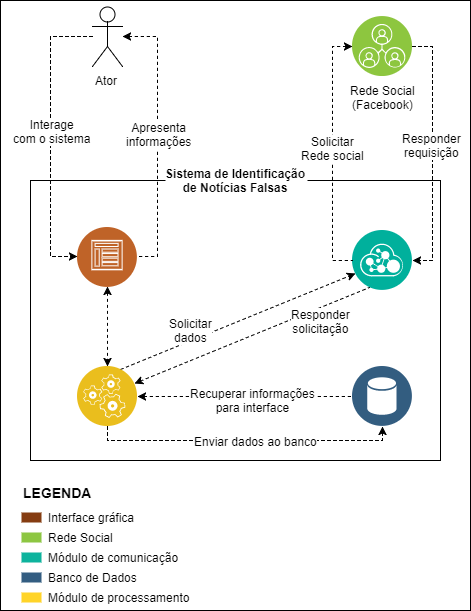
\includegraphics[scale=0.6]{4-proposta/arquitetura_do_sistema.png}
\caption{Arquitetura do sistema de identificação coletiva de notícias falsas.}
\label{fig:arquitetura_sist_id_not_falsas}
\end{figure}

\subsection{Interface gráfica}
Este elemento da arquitetura deve prover suporte ao usuário em termos de execução das operações dentro do sistema e de apresentação dos resultado das suas ações. As operações básicas planejadas de acordo com o modelo teórico são:

\begin{itemize}
    \item atribuir/remover autoridade cognitiva a um ator;
    \item inserir/buscar objeto (URL)
    \item organizar autoridade cognitiva recebida, incluindo aceitação/negação e auto-atribuição e remoção completa
    \item requisitar opinião de ator em relação a um objeto
    \item inserir/remover palavras-chave em um objeto
    \item inserir/remover classificação de um objeto
\end{itemize}

\subsection{Rede social}
Segundo \cite{nic.br_pesquisa_2017} o \emph{Facebook} e o \emph{Twitter} são as duas redes sociais mais populares no Brasil, neste trabalho optamos por focar no \emph{Facebook} pois além do grande público alcançado pela plataforma online, a empresa também detém o domínio de dois aplicativos de mensagens (\emph{Facebook Messenger e Whatsapp}), que de acordo com \cite{nic_newman_digital_2017} possuem um grande crescimento no Brasil. Portanto, neste trabalho utilizaremos a rede social do \emph{Facebook} para aplicar nosso modelo. Isso será possível graças a uma API (chamada \emph{The Graph API}) desenvolvida pela empresa. A \emph{Graph} proporciona formas de acesso ao gráfico social de usuários cadastrados (com devidas permissões) possibilitando recuperação de informações destes usuários, entre essas poderemos extrair a lista de amigos e informações públicas que caracterizam seus perfis online;
   
\subsection{Módulo de comunicação}
Este módulo recebe do solicitações do módulo de processamento, essas serão enviadas a um serviço externo. Neste trabalho esse módulo será o intermediário entre o protótipo e a rede social;
    
\subsection{Módulo de processamento}
É responsável pelo processamento das requisições realizadas pelo usuário na interface gráfica, por recuperar e inserir informações do banco de dados quando necessário, somar de autoridade cognitiva dos atores, somar o índice de classificação e palavras-chave dos objetos e requisitar ao módulo de comunicações informações das APIs externas; 
    
\subsection{Banco de dados}
É responsável pela persistência das informações e entidades que serão utilizados no sistema. Esse elemento é de grande importância, pois a modelagem das tabelas do banco de dados irão definir como iremos armazenar e recuperar as informações, tanto para a operação do sistema. A figura \ref{fig:mer} ilustra quais são as principais entidades existentes e como as tabelas do banco irão se relacionar. Observa-se que temos 4 entidades principais, com mais duas tabelas auxiliares totalizando 6 tabelas listadas, cada uma responsável pelo armazenamento de uma entidade no nosso sistema: 

    \begin{figure}[ht]
    \centering
    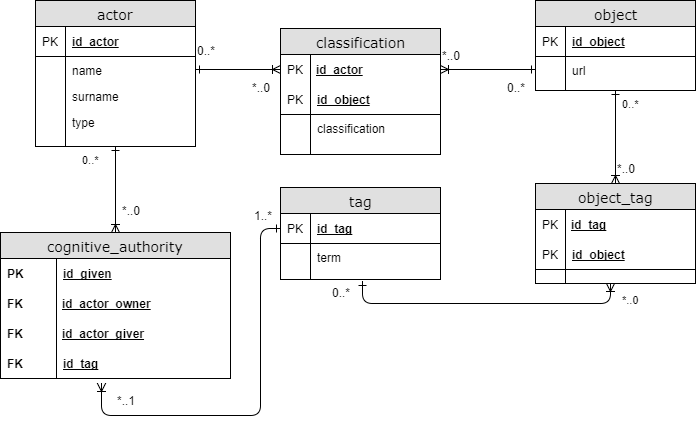
\includegraphics[scale=0.5]{4-proposta/mer.png}
    \caption{Modelo entidade relacionamento do banco de dados.}
    \label{fig:mer}
    \end{figure}

\begin{enumerate}
    \item \textbf{\emph{Actor} (Ator)}: representa os atores do sistema, possui os atributos \emph{id\_actor} (identificador único), \emph{name}(nome), \emph{surname} (sobrenome) e \emph{type}(tipo). O atributo \emph{type} é relativo ao tipo de ator, podendo representar, pessoa física, artista, instituição ou organização. Os outros atributos são auto-explicativos e foram idealizados apenas para propósito de identificação, porém outros atributos podem ser interessantes, como endereço, educação, entre outros. 
    
    Além dos atributos, a tabela \emph{actor} possui dois relacionamentos, um de zero para muitos com a tabela \emph{cognitive\_authority}, representando que cada entidade ator possui zero ou mais entidades de autoridades cognitivas concebidas e/ou recebidas. E um de muitos para muitos com a tabela \emph{object}, representando que um ator pode classificar zero ou mais objetos, que por sua vez, podem ser classificados por zero ou mais atores ;
    
    \item \textbf{\emph{Cognitve authority}}: esta tabela representa uma autoridade cognitiva recebida ou concedida, possui os seguintes atributos: 
    \begin{itemize}
        \item \emph{id\_received}: identificador único da tabela;
        \item \emph{id\_actor\_owner}: identificador de quem recebeu a autoridade cognitiva;
        \item \emph{id\_actor\_giver}: identificador do ator que concedeu a autoridade cognitiva; 
        \item \emph{id\_tag}: é o identificador único de uma \emph{tag} (rótulo); 
    \end{itemize}
    
    \item \textbf{\emph{Tag}}: é a entidade responsável pelos rótulos dos objetos e das AC no sistema cada \emph{tag} possui uma identificação única (\emph{id\_tag}, e um atributo queem uma cas armazenará o termo utilizado na rotulação (\emph{term}). Os relacionamentos presentes nesta tabela são com as tabelas  \emph{cognitive\_authority} e \emph{object\_tag}. A primeira é uma relação de um para muitos onde uma autoridade cognitiva dada ou recebida possui apenas um rótulo que a descreve. A segunda é uma relação muitos para muitos com a entidade \emph{object}, demonstrando que um rótulo pode estar presente em vários objetos distintos e um objeto pode conter vários rótulos distintos. Para possibilitar este relacionamento foi utilizado a entidade auxiliar \emph{object\_tag};
    
    \item \textbf{\emph{Object}}: esta entidade é responsável por armazenar dados sobre o objeto proposto no modelo, possui os seguintes atributos:
    \begin{itemize}
        \item \emph{id\_object}: é o identificador único do objeto;  
        \item \emph{url}: é a forma padronizada que foi escolhida para a representação da informação no sistema, este formato foi escolhido por sua ampla gama de usos, podendo representar documentos, sites, artigos, fotos, entre outros;
    \end{itemize}
    A tabela possui dois relacionamentos de muitos para muitos com as tabelas \emph{actor} e \emph{tag} , o primeiro  sinaliza que um ator pode classificar zero ou mais objetos que, podem ser classificados por zero ou mais atores. O segundo, mostra que um objeto possui zero ou mais rótulos que podem ser utilizados para descrever zero ou mais objetos. Essas relações se fazem possíveis pela utilização das tabelas auxiliares: \emph{obect\_tag} e \emph{classification}.
\end{enumerate}    

% --------------------------------------------------------------------------------------------------------------------

\section{Avaliação}

Pesquisas cientificas são realizadas visando o progresso ou aperfeiçoamento. Portanto, devem existir maneiras de quantificar esse progresso. De acordo com \cite{jayaratna_understanding_1994} nenhum processo, que visa a solução de um problema, pode ser considerado completo até que uma avaliação deste seja realizada. É esta avaliação que irá auxiliar na medição da efetividade da solução em frente ao problema encontrado. Se este elemento não for considerado, é impossível saber ao certo se o problema foi solucionado em algum nível.

\subsection{Abordagens de pesquisa}

Segundo \cite{chen_s._information_2011}, em pesquisas de avaliação podemos utilizar abordagens quantitativos, qualitativos e a mistura dos dois. \cite{creswell_research_2014} comenta que essas abordagens não são opostas, argumentado que um estudo pode ser mais qualitativo que quantitativo e vice-versa. Ele define as três abordagens da seguinte forma:

\begin{itemize}
    \item Pesquisa \textbf{qualitativa}: é um meio para explorar e entender o significado que os indivíduos ou grupos atribuem a um problema social ou humano. O processo de pesquisa envolve questões e procedimentos emergentes, os dados normalmente são coletados a partir da configuração de um participante. A análise de dados é construída de forma indutiva de temas particulares para gerais. E o pesquisador realiza suas interpretações do significado dos dados. O relatório final possui uma estrutura flexível. Aqueles que se envolvem nesta forma de inquérito apoiam um olhar um estilo indutivo de fazer pesquisa, com um foco no significado individual e na complexidade de uma situação (\cite{creswell_research_2014}).
    
    \item Pesquisa \textbf{quantitativa}: é um meio para testar teorias objetivas examinando a relação entre variáveis. Essas variáveis por sua vez, podem ser medidas, tipicamente com instrumentação, de modo que os dados possam ser analisados usando procedimentos estatísticos. O relatório escrito final possui uma estrutura definida que consiste em introdução, literatura e teoria, métodos, resultados e discussão. Aqueles que se envolvem nesta forma de investigação testam suas teorias de forma dedutiva, constroem proteções contra viés, controlam explicações alternativas e são capazes de generalizar e replicar suas descobertas (\cite{creswell_research_2014}).
    
    \item Pesquisa com \textbf{métodos mistos}: é uma abordagem de investigação que combina ou associa ambas as formas mostradas: qualitativas e quantitativas. Envolve pressupostos filosóficos, o uso de abordagens qualitativas e quantitativas e a mistura de ambas as abordagens em um estudo. Portanto, é mais do que simplesmente coletar e analisar ambos os tipos de dados, é o envolvimento de ambas as abordagens em conjunto, de modo que a força geral de um estudo seja maior do que a pesquisa qualitativa ou quantitativa (\cite{creswell_research_2014}).
\end{itemize}

Como forma de auxilio para a escolha da abordagem de pesquisa \cite{creswell_research_2014} apresenta um \emph{framework} relacionando três componentes: visões filosóficas do mundo; estratégias de investigação e métodos específicos. As quatro visões de mundo, segundo \cite{creswell_research_2014} são:

\subsection{Visões filosóficas}

\begin{enumerate}
    \item \textbf{Pós-positivismo}: Os pressupostos pós-positivistas representaram a forma tradicional de pesquisa, e essas são mais relacionadas a pesquisas quantitativas do que qualitativas. É chamado de pós-positivismo porque representa o pensamento após o positivismo, desafiando a noção tradicional da verdade absoluta do conhecimento e reconhecendo que não podemos ser "positivos" sobre nossas reivindicações de conhecimento ao estudar o comportamento e as ações dos seres humanos. Os problemas estudados pelos pós-positivistas refletem a necessidade de identificar e avaliar as causas que influenciam os resultados (\cite{creswell_research_2014});

    \item \textbf{Construtivismo}: Os construtivistas detêm pressupostos de que os indivíduos buscam a compreensão do mundo em que vivem e trabalham. Os indivíduos desenvolvem significados subjetivos de suas experiências. Essa perspectiva tem maior relação com uma abordagem qualitativa de pesquisa (\cite{creswell_research_2014});
    
    \item \textbf{Advocacia/Participativa}: Este grupo de pesquisadores detém os pressupostos filosóficos da abordagem advocacia / participação. Esta posição surgiu durante os anos de 1980 e 1990, fundamentada por indivíduos que sentiram que os pressupostos pós-positivistas impunham leis e teorias estruturais que não se encaixavam em indivíduos marginalizadas da nossa sociedade. Esta visão de mundo é normalmente vista com pesquisa qualitativa, mas pode ser utilizada como uma base para a pesquisa quantitativa (\cite{creswell_research_2014});
    
    \item \textbf{Pragmatismo}: O pragmatismo como visão de mundo surge de ações, situações e consequências, em vez de condições antecedentes (como no pós-positivismo). Existe uma preocupação com as aplicações, com o que funciona e as soluções para os problemas. Em vez de se concentrar em métodos, os pesquisadores enfatizam o problema da pesquisa e usam todas as abordagens disponíveis para entender o problema. Tem maior relação com os estudos de métodos mistos (\cite{creswell_research_2014}).
\end{enumerate}

Os principais elementos dessas visões de mundo podem ser observados na tabela \ref{tab:visoes_mundo}.

    \begin{center}
        \begin{table}[!htp]
            \caption{Diferentes visões de mundo e seus elementos}
            \label{tab:visoes_mundo}
            \begin{tabular}{|p{4.5cm}|p{10cm}|}
                \cline{1-2}                                 
                \hline
                {Pós-positivismo}                        &$\bullet$ Determinismo                             \\
                                                         &$\bullet$ Reducionismo                             \\
                                                         &$\bullet$ Observação empírica e medição            \\
                                                         &$\bullet$ Verificação de uma teoria                \\
                \hline
                {Construtivismo}                         &$\bullet$ Compreendimento                          \\
                                                         &$\bullet$ Múltiplos significados dos participantes \\
                                                         &$\bullet$ Construção social e histórica            \\
                                                         &$\bullet$ Geração de uma teoria                    \\
                \hline
                {Advocacia/Participativa}                &$\bullet$ Política                                 \\
                                                         &$\bullet$ Problema orientado a empoderamento       \\
                                                         &$\bullet$ Colaborativo                             \\
                                                         &$\bullet$ Orientado a mudança                      \\
                \hline
                {Pragmatismo}                            &$\bullet$ Consequência de ações                    \\
                                                         &$\bullet$ Centralizado em torno do problema        \\
                                                         &$\bullet$ Pluralismo                               \\
                                                         &$\bullet$ Orientado a práticas do mundo real       \\
                \hline
            \end{tabular}
        \end{table}
    \end{center}

\subsection{Estratégias de investigação}

Um pesquisador ainda deve ponderar sobre as estratégias de investigação que irá utilizar em sua pesquisa. Essas estratégias são designs ou modelos que fornecem uma direção específica para os procedimentos que serão realizados no design da pesquisa. \cite{creswell_research_2014} relaciona essas estratégias com suas abordagens de pesquisa, assim como ilustrado na tabela \ref{tab:estrategias_investigacao}.

    \begin{center}
        \begin{table}[!htp]
            \caption{Estratégias de investigação e abordagens de pesquisa}
            \label{tab:estrategias_investigacao}
            \begin{tabular}{|p{4.5cm}|p{5cm}|p{5cm}|}
                \hline
                Quantitativo                      & Qualitativo                     & Métodos mistos   \\
                \hline
                Designs Experimentais;              & Pesquisa de Narrativa;          & Sequencial; \\
                Designs não-experimentais, como entrevistas.     & Fenomenologia;       & Concorrente;    \\
                                                  & Etnografias;       & Transformativo.    \\
                                                  & Estudo de teorias fundamentadas;       &     \\
                                                  & Estudo de caso.       &     \\
                \hline
            \end{tabular}
        \end{table}
    \end{center}

\subsection{Métodos de pesquisa}

O terceiro elemento principal do \emph{framework} de \cite{creswell_research_2014} é o método de pesquisa, que envolve as formas de coleta, análise, e interpretação dos dados que os pesquisadores propõem nos seus estudos. A tabela \ref{tab:metodos_pesquisa} ilustra os métodos de pesquisa discutidos por \cite{creswell_research_2014}.

    \begin{center}
        \begin{table}[!htp]
            \caption{Métodos e abordagens de pesquisa}
            \label{tab:metodos_pesquisa}
            \begin{tabular}{|p{4.5cm}|p{5cm}|p{5cm}|}
                \hline
                Quantitativo                      & Qualitativo                     & Métodos mistos   \\
                \hline
                Pré-determinados              & Métodos emergentes          & Ambos \\
                \hline
                Questões baseadas fechadas com respostas diretas & Questões abertas       & Ambos    \\
                \hline
                Dados de performance, atitude, de observação e de censo  & Dados de entrevistas, de observação, de documentos e áudio-visual       &  Todas as possibilidades    \\
                \hline
                Análise estatística & Análise textual e de imagens       &  Ambas   \\
                \hline
                Interpretação estatística  & Interpretação de temas e padrões       & Ambas    \\
                \hline
            \end{tabular}
        \end{table}
    \end{center}

\subsection{Estratégia de pesquisa proposta}

Baseado nas características apresentadas no estudo de \cite{creswell_research_2014}, foi identificado que este estudo utilizará uma abordagem quantitativa de pesquisa e portanto se utilizará dos métodos quantitativos citados. Portanto, foi escolhido o seguinte cenário:

\begin{itemize}
    \item Visão filosófica: Pós-positiva ;
    \item Estratégia de investigação: Entrevistas e experimentos;
    \item Métodos de pesquisa: Entrevistas com questões fechadas, experimentos com cenários pré-determinados, e extração de dados numéricos;
    \item É responsabilidade do pesquisador: Testar a teoria, identificar de variáveis de estudo, relacionar de variáveis em questões e hipóteses, utilizar padrões de validade e confiabilidade, observar e avaliar informações numericamente, utilizar uma abordagem imparcial, empregar procedimentos estatísticos.
\end{itemize}